\documentclass[tikz,border=3mm]{standalone}
\usepackage{amsmath,amssymb}
\usetikzlibrary{arrows.meta,positioning}

\begin{document}
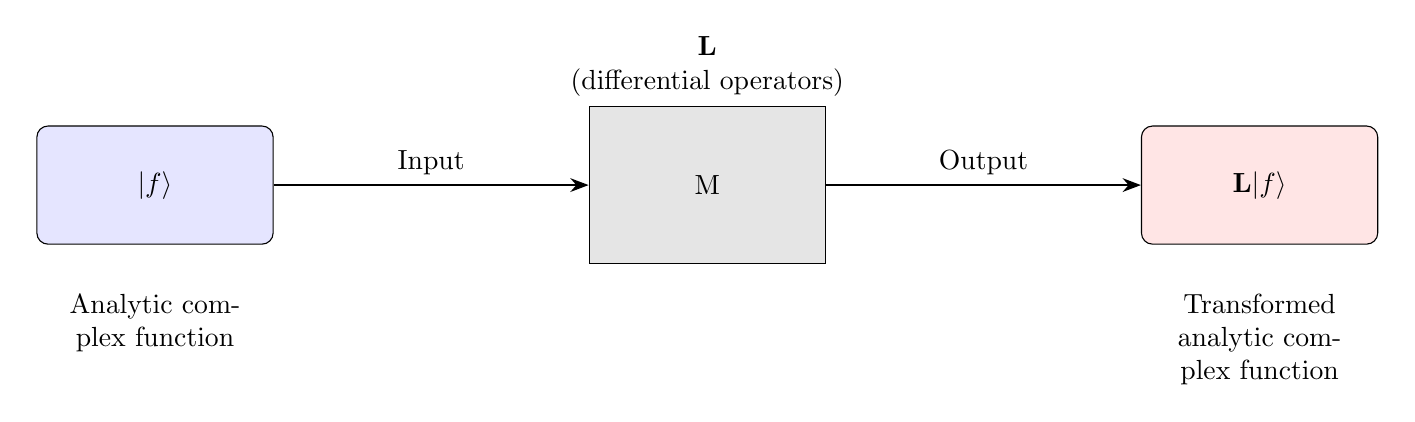
\begin{tikzpicture}[
    node distance=4cm,
    func/.style={draw, rounded corners, fill=blue!10, minimum width=3cm, minimum height=1.5cm},
    machine/.style={draw, rectangle, fill=gray!20, minimum width=3cm, minimum height=2cm},
    op/.style={above, align=center, font=\boldmath},
    >=Stealth
]

% Input function
\node[func] (input) {$|f\rangle$};

% Machine with operator
\node[machine, right=of input] (machine) {M};
\node[op] at (machine.north) {$\mathbf{L}$\\(differential operators)};

% Output function
\node[func, right=of machine, fill=red!10] (output) {$\mathbf{L}|f\rangle$};

% Arrows with labels
\draw[->,thick] (input) -- node[above] {Input} (machine);
\draw[->,thick] (machine) -- node[above] {Output} (output);

% Annotation
\node[below=5mm of input, anchor=north, text width=3cm, align=center] 
    {Analytic complex function};
\node[below=5mm of output, anchor=north, text width=3cm, align=center] 
    {Transformed analytic complex function};

\end{tikzpicture}
\end{document}